\documentclass[a4paper]{article}

\usepackage[swedish]{babel}
\usepackage[T1]{fontenc}
\usepackage[utf8]{inputenc}
\usepackage{ graphicx }

\begin{document}
\begin{center}
\thispagestyle{empty}
\parskip=14pt%
\vspace*{3\parskip}%

{\LARGE Projektplan DAT290}

{\large Larmsystem, grupp 11

Fredrik Österström, Lukas Schiavone, Markus Moen, Nazif Kadirogl, Titus Blosse, Viktor Frideen

\today}


\rule{7cm}{0.4pt}\\
\end{center}
\newpage

\thispagestyle{empty}
\tableofcontents
\newpage

\pagenumbering{arabic} 

Ni skriver all text i projektplanen med ett projektinternt perspektiv.
Detta betyder att ingenstans ska det framgå att projektet drivs inom
ramen för en kurs i utbildningssyfte, utan att detta är ett rent
tekniskt utvecklingsprojekt.

Eftersom de tre första avsnitten, Syfte, Mål och Bakgrund, återkommer
(helt intakta, om de är välskrivna) i projektrapporten, tveka inte över
att ägna ordentligt med tid åt dessa.



\section{SYFTE}


Syftet beskriver koncist varför projektet ska genomföras och vad ett
uppfyllande av de tekniska målen leder till.

Vanligtvis är syftet så klart ledande för uppgiften man löser. Här är
det lite tvärt om eftersom ni fått en uppgift och måste komma på ett
syfte för den, men det ska nog gå bra.

Ha gärna med lite fakta i syftesparagrafen. Istället för att bara skriva
självklarheter som att det är bra med larm ifall det kommer tjuvar så
kan man ha med några siffror på vad larmbranchen omsätter till exempel
eller hur vanligt det är med inbrott eller något.



\section{MÅL}


I detta avsnitt beskrivs koncist samtliga övergripande tekniska mål med
projektet, det vill säga, vad ska konstrueras. Mycket av det här
framgår så klart i uppgiften.

Se till att tydligt ange målsättningen vad gäller de extrauppgifter som
finns tillgängliga i projektdirektiven. Ni kan dela upp eventuella
extrauppgifter i två olika prioritetsgrader. Att ta på sig en massa
extrauppgifter här som ni inte ens försöker genomföra är inte bra.
Försök göra en realistisk bedömning av vad ni hinner med även om det är
svårt.

De mål som anges här kommer att styra projektets utveckling. När
projektet närmar sig sitt slut och den slutliga projektrapporten lämnas
in kommer beställaren (läraren i vårt fall) att kritiskt analysera hur
väl projektet lyckats genom att jämföra planens mål med den tekniska
konstruktion som redovisas i projektrapporten.



\section{BAKGRUND}


Genom att det fyller i de kompetensluckor som en typisk läsare har,
underlättar bakgrundstexten läsandet av konstruktionsavsnitten. Precis
som avsnitten Syfte och Mål ovan kan detta avsnitt med fördel
återanvändas i den slutgiltiga projektrapporten. När det gäller
projektplanen för DAT290 beskrivs här bakgrunden till projektet vad
gäller tillämpningen, dess sammanhang och de tekniska förutsättningar
som råder. För att beskriva tillämpningen och dess sammanhang behöver ni
förklara hur system av den typen som ska konstrueras här fungerar i
största allmänhet.

Men vem är den typiska läsaren? Man får förutsätta att läsaren har en
viss teknisk kompetens, annars blir bakgrundsavsnittet alltför långt.
Denna gränsdragning (“hur elementärt ska jag förklara vad jag gör?”)
upplevs som ett svårt moment när man som student börjar skriva tekniska
rapporter. En användbar regel är att vi utgår från att läsaren har, i
stort sett, samma utbildning som rapportskribenten, men saknar
specialistkunskap om projektets tillämpning.


\subsection{Referenser}

I regel använder bakgrundsavsnittet olika källor (eller referenser) för
att bygga under resonemang som skribenten för. Man kan som sagt vilja
hänvisa läsaren till en källa för att underbygga ett påstående, men det
kan också handla om att hänvisa läsaren till en källa som ger mer
information om något man tar upp i förbigående (se referensen kring IEEE
som jag ger nedan). Det finns flera olika system för hur referenser
hanteras. Bland de mest kända återfinns Harvard och Oxford; medan det
förra använder en referenslista i slutet av dokumentet, använder det
senare sig av en not/fotnot per referens, löpande i texen. I DAT290
använder vi referenssystemet som organisationen IEEE tagit fram \cite{Hughen}. Detta
är ett Harvard-likt referenssystem där man samlar alla referenser i en
avslutande numrerad förteckning till vilken man hänvisar med referensens
nummer. Valet av detta referenssystem beror på att IEEE publicerar många
journaler inom datortekniksområdet och att det är ett vanligt system för
våra kandidat- och examensarbeten.

Bra referenser är till exempel kurslitteratur eller andra akademiska
böcker. Akademiska artiklar är också bra referenser, särskilt för mer
specifika påståenden. I bästa fall så ska alla påståenden som inte är
helt uppenbara ha källhänvisningar.


\subsection{Tekniska förutsättningar}

När det gäller tekniska förutsättningar så behöver ni förtydliga vad som
är givet i projektet: Beskriv övergripande vilken hårdvara och mjukvara
som kan förutsättas och vad som ska nyutvecklas. Som ni senare kommer
upptäcka överlappar denna beskrivning till viss del med resursplanen i
avsnitt \ref{sec:RESURSPLAN}. I och med att detta sista avsnitt skiljer sig
ganska mycket från tillämpningsgenomgången ovan kan det här vara läge
att använda sig av en underrubrik.



\section{SYSTEMÖVERSIKT}


För att konkretisera en struktur som ett datorsystem underlättar det
ofta att rita en figur, till exempel ett blockschema, över systemet som
man tänker sig att implementera. I detta avsnitt beskriver ni
översiktligt systemet, lämpligen genom en (eller flera) figur(er). Se
till att hänvisa till figuren från texten och att använda en rubrik för
figuren. Eftersom systemet är ganska komplext behöver ni tänka igenom
vilken detaljrikedom systemöversikten ska ha; dels känner ni ännu inte
till detaljer eftersom konstruktionsarbetet inte påbörjats, dels skulle
inte alla detaljer få plats i en figur över systemet.

I och med att det finns ett grundsystem till vilket man kan lägga
kompletteringar behöver era val av kompletteringar beskrivas
översiktligt. Om ni avser att arbeta med egendefinierade kompletteringar
krävs en mer detaljerad beskrivning än om ni använder kompletteringar
som beskrivs i projektdirektivet.

Under projektets genomförande kommer ni att få anledning att revidera
figuren över systemet. Att ta fram den ultimata figuren över det
slutliga systemet är varken möjligt eller önskvärt under
planeringsfasen, utan det är framförallt processen med att ta fram
figuren som är viktig eftersom denna process hjälper gruppen att
fokusera tänkandet, att skapa gemensamma tekniska ramar och att rensa
bort (en del) tekniska oklarheter.



\section{RESURSPLAN}
\label{sec:RESURSPLAN}


Gör en lista över gruppmedlemmarna och ange tydligt hur man kommunicerar
med var och en av dessa (till exempel, ange epostadresser).
Utgångspunkten är att alla gruppmedlemmar är tillgängliga genom hela
projektet. Om det finns undantag, ange dessa.

Ange vilka roller som de olika gruppmedlemmarna har. Det är lämpligt att
en person är ansvarig för ett distinkt område; delat ansvar är
komplicerat. Här är ett förslag på ansvarsområden inom gruppen. Andra
områden är möjliga, till exempel kan man dela upp ansvaret för olika
delar av projektet istället för olika (men var försiktig med det för det
kan leda till att gruppen blir splittrad). Notera att ansvaret inte
innebär att man gör mer av det praktiska, snarare att övervakar gruppens
arbete och uppmärksammar gruppen när något inte fungerar.

\begin{itemize}
    \item Gruppledare: Ansvarar för kommunikation med kursens lärare, ansvarar
    för att kalla till och leda gruppmöten.

\item Administrativt dokumentationsansvarig: Ansvarar för att
    mötesprotokoll förs. Ansvarar för att gruppen i tid börjar på
    oppositionsrapport, planeringsrapport och så vidare och ansvarar för
    att dessa skickas in i tid.

\item Teknisk dokumentationsansvarig: Ser till att kod är väl kommenterad.
    Uppmärksammar gruppen ifall det uppstår problem med kod som inte är
    tillräckligt dokumenterad.

\item Kodstandardansvarig: Kollar igenom att all kod som utvecklas följer
    standarder för struktur, namn och så vidare som gruppen bestämt.
    Uppmärksammar gruppen ifall disciplinen behöver skärpas vad
    gäller kodkvalitet.

\item Testansvarig: Håller ordning på de olika test som behöver genomföras
    på mjukvara och hårdvara, ser till att tillräcklig tid ägnas åt
    testning och att den dokumenteras väl. Uppmärksammar gruppen ifall
    testningen inte utförs eller dokumenteras tillräckligt.

\item Resursansvarig: Ser till att hårdvaran finns tillgänglig när den
    behövs, ansvarar för att olika verktyg ni använder för
    kommunikation, versionshantering och så vidare fungerar och
    används korrekt. Uppmärksammar gruppen ifall verktygen används fel
    eller inte fungerar väl.

\item Planeringsansvarig: Håller reda på de olika del-mål gruppen arbetar
    mot, kommunicerar med de andra gruppmedlemmarna om hur arbetet med
    dessa fortskrider och ger en rapport om det på veckomöten.
    Uppmärksammar gruppen så tidigt som möjligt om något mål inte gör
    framsteg så att gruppen kan planera om ifall det behövs eller så att
    arbetsinsatser kan omfördelas.
    
\end{itemize}

\begin{table}[]
\centering
\begin{tabular}{|l|l|l|}
\hline
    Nr & Beskrivning & Datum \\
    \hline
    1 & Projektplan inlämnad & 2020-09-13 \\
    \hline
    .. & ... & ... \\
    \hline
    .. & Grundsystem verifierat & 2020-XX-XX \\
    \hline
    .. & GUI-programmering avslutad & 2020-XX-XX \\
    \hline
     
\end{tabular}
\caption{Milstolpar för projektet}
\label{milstolpar}
\end{table}

Ange vilka lokaler som kan disponeras, och när. Ange vilken hårdvara och
vilken mjukvara som finns tillgänglig. I och med att en del hårdvara
görs tillgänglig på begäran, ange hur ni begär ut hårdvara.

Om gruppmedlemmar vill arbeta med projektet på distans, utanför
Chalmers, beskriv hur man lämpligen går tillväga.





\section{MILSTOLPAR}


Här ska ni ange ett urval av de mest signifikanta målen som stöd till
projektuppföljningen. Är milstolparna för många ger de inget stöd till
projektstyrningen; som tumregel kan ni använda en till två milstolpar
per vecka.

Det är viktigt att man väljer mål som är mätbara, till exempel kan man
använda sig av “Grundsystem verifierat” eller “GUI-programmering
avslutad”. De inlämningar ni behöver göra ska så klart ingå som
milstolpar men det kan även vara bra att i gruppen besluta om att de ska
vara i princip färdiga en viss tid innan deadline. Ett exempel på hur
milstolparna kan presenteras ges i tabell [tab:milstolpar].

\section{AKTIVITETER}


Här ger ni en detaljerad beskrivning av arbetspaket/arbetsuppgifter
kopplat till total tidsåtgång per paket. Tidsåtgången är alltså inte per
medlem utan det är en total siffra (“mantimmar”) för alla som är
involverade i just denna aktivitet. En kurs om 7,5 p motsvarar ju 200
timmar per student. I grupper om sju eller åtta personer finns det
alltså totalt 1400 eller 1600 timmar att disponera till olika
aktiviteter.

När ni sitter och skriver på denna lista vet ni ju exakt hur många
timmar som redan använts (och ja, dessa timmar ska också skrivas ned!)
men för veckorna framgent måste ni gissa. Ett exempel på de första
raderna i en aktivitetslista ges i tabell [tab:aktiviteter].

Eftersom ni förr eller senare ska matcha aktiviteter till medlemmar är
ett tips att ni skriver upp vilken eller kanske snarare vilka
gruppmedlemmar som hör ihop med respektive aktivitetet. Med denna
planering blir det sedan möjligt för gruppen att följa upp arbetet i de
veckovisa projektgruppsmötena.



\section{TIDSPLAN}

\begin{table}[]
    \centering
\begin{tabular}{ |c|c|c| } 
 \hline
 1 & Första genomläsning mikrodatordokumentation & 20 h\\ 
 \hline
 2 & Framtagning av LaTeX-mallar & 6 h \\ 
 \hline
 3 & Projektmöten (2h/vecka, 8 veckor, 7 personer)  & 112 h \\ 
 \hline
 4 & Projektledning (3h/vecka, 8 veckor) & 24 h \\ 
 \hline
 5 & Dokumentgranskning & 8 h \\
 \hline
 6 & Programmering av API/drivrutin USART & 100 h\\ 
 \hline
 7 & Programmering av högpassfilter & 80 h \\ 
 \hline
 8 & Dimensionering/konstruktion förstärkare & 150 h \\ 
 \hline
 .. & ... & ... \\ 
 \hline
 .. & Skriv oppositionskommentar & 8 h \\ 
 \hline
 .. & Förbered/genomför demonstration & 40 h \\
 \hline
 .. & Arbeta med projektrapport & ... \\ 
 \hline
\end{tabular}
\caption{Aktivitetslista för projektet}
\label{Aktivitetslista}
\end{table}

\begin{figure}
    \centering
    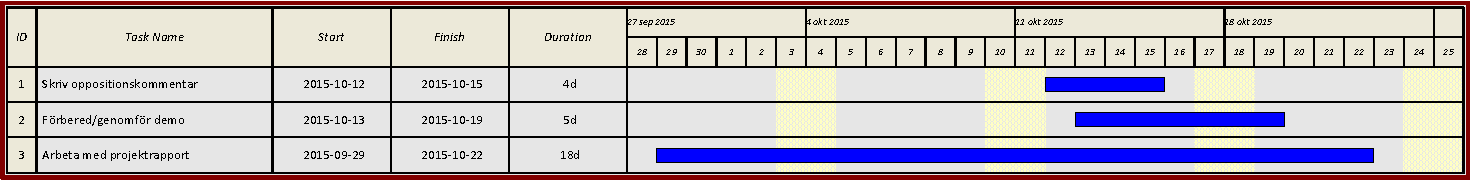
\includegraphics[width=\textwidth]{tidsplan.pdf}
    \caption{En skiss på en Ganttbased tidsplan för de senare läsveckorna.}
    \label{fig:my_label}
\end{figure}

Det kommer periodvis att finnas flera olika aktiviteter som löper
parallellt. Ta till exempel läsvecka 7 och 8 där 1) en
oppositionskommentar för en annan grupps projektrapportsutkast ska
skrivas, 2) en demonstration av slutprodukten ska förberedas och
genomföras, och 3) en projektrapport v. 1 ska avslutas. Med en grupp om
sju-åtta personer bör man planera så att dessa aktiviteter på ett
smidigt sätt löper parallellt. Ett Ganttschema (se figur [fig:Gantt])
kan illustrera de olika aktiviteterna (och möjligen även milstolparna)
på en horisontell tidslinje.

[En skiss på en Ganttbased tidsplan för de senare läsveckorna.]

Om man kan koppla de olika aktiviteterna till gruppmedlemmar (risken
finns att Ganttschemat kan bli rörigt) finns det en möjlighet att
urskilja kritiska beroenden mellan olika delar av projektet.



\section{MÖTESPLAN}


Ange datum, tid och lokal för de veckovisa projektmötena som involverar
hela gruppen samt mentorn. Ange även, så långt det är möjligt, datum,
tid och lokal för mer specialiserade arbetsmöten.



\section{KOMMUNIKATIONSPLAN}


Det blir en hel del skrivande i ett projekt. För större projekt är
kommunikationen så komplex att det är värt att tydligt definiera en plan
över all skriftlig kommunikation. Man kan exempelvis presentera det som
i tabell \ref{tab:kommunikationsplan} (där PP står för PingPong, och Alla
betyder grupp, mentor och lärarteam).

\begin{table}[]
    \centering
    \begin{tabular}{|l|l|l|l|}
    \hline
        Vad & När & Till & Hur \\ 
        \hline
        \hline
        Dagordning möte LV1 & 2020-09-02 & Alla & PP loggbok (som text) \\ 
        \hline
        Mötesprotokoll möte LV1 & 2020-09-04 & Alla & PP loggbok (som text) \\
        \hline
        Projektplan & 2020-09-11 & Lärarteam & PP inlämning (latex) \\
        \hline
        ... & ... & ... & ... \\
        \hline
        Projektrapport & 2020-10-22 & Lärarteam & PP inlämning (latex) \\
        \hline
    \end{tabular}
    \caption{Kommunikationsplan för projektet}
    \label{tab:kommunikationsplan}
\end{table}

Här har jag utgått från att det finns 1) en dokumentationsansvarig som
ser till att dokument som projektplan och projektrapport i rätt tid
sänds till rätt adressat och 2) en projektledare som ser till att
dagordning och mötesprotokoll läggs upp på PingPong.

Se även till att ni tidigt enas om hur ni kommunicerar inom gruppen:
Ni har visserligen tillgång till en grupplogg inom PingPong där ni kan
beskriva era framsteg, men ni behöver dessutom ha någon slags
peer-to-peer-kommunikation.



\section{KVALITETSPLAN}


Beskriv era rutiner för att verifiera respektive delsystem och, i
slutändan, hela systemet. Ni kan till exempel använda en enkel
verifieringsmall som ska fyllas i samband med att en del av systemet
verifieras: Här kan man tänka sig rubriker som

\begin{desctription}

\item[Komponent] Vilken del av systemet ska testas?

\item[Testsyfte] Vad ska testet visa?

\item[Utförande] Hur ska testet utföras? Vilka scenarior testas?

\item[Resultat] Vad är testresultatet?

\item[Analys] Vad innebär testets resultat? Behövs fler test av komponenten? Behöver andra komponenter testas ytterligare?
\end{desctription}

Tänk på att olika delar av systemet behöver olika verifieringsmetodik;
medan mjukvara kan verifieras i det IDE (Integrated Design Environment)
som ni använder, behöver ni använda mätutrustning för elektronik.


\section{SPELREGLER}


Denna rubrik kring spelregler är helt frivillig eftersom den normalt
sett inte ingår i en projektplan. Skälet för att ha med spelregler här
är att göra er överenskommelse kring dessa synlig och tydlig. Följden är
att att ingen gruppmedlem senare kan säga att han eller hon inte är
införstådd med dessa. Det kan handla om någonting så simpelt som vad
konsekvensen är av att någon kommer för sent till ett möte. Men det kan
också handla om mer allvarliga saker som att någon enskild medlem inte
levererar material vid en tidpunkt som gruppen bestämt i projektplanen.


\bibliographystyle{ieeetr}
\bibliography{referenser}
\end{document}
